

\begin{figure}
\begin{mdframed}[backgroundcolor=gray!04] 
\begin{scriptsize}

{\large \textbf{Task: Titanic}} \bigskip


Data about passengers on the Titanic offer an interesting yet simple scenario for data manipulation, filtering, and visualization. \medskip


For this particular dataset, each row provides information in the following format:

\medskip

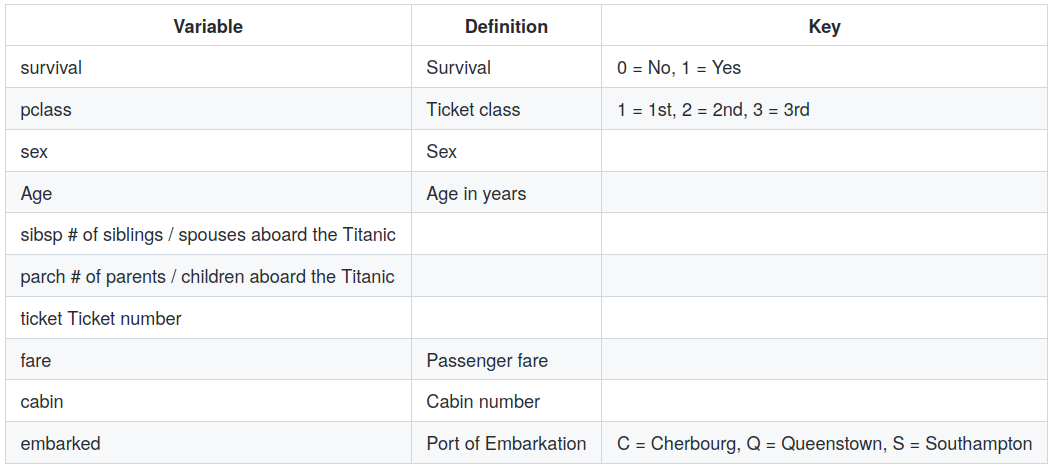
\includegraphics[width=\textwidth]{appendix/cp6/titanic-table.png}

\medskip




\begin{center}
\rule{10cm}{0.4pt}
\end{center}

\textbf{Task} \medskip

Given a \code{string} representing a url for the titanic dataset (in \code{csv} format), you must write an algorithm using the \code{pandas} and \code{seaborn} modules to create a barchart with the passengers' average fare according to the following constraints \medskip


Constraints:

\begin{itemize}


    \item Passengers age must be \code{>= 18}

    \item  Passengers age must be \code{<= 30}

    \item Averages are affected by outliers, so you must ignore fares \code{>= 100}

    \item  The only variables of interest are \code{sex}, \code{age}, and \code{fare}

    \item You must return a call to \code{seaborn.barplot} so that tests can plot the chart and check the values in the \code{x-axis} and \code{y-axis} according to the data.


\end{itemize}

\end{scriptsize}
\end{mdframed}
\end{figure}
  


\begin{figure}
\begin{mdframed}[backgroundcolor=gray!04] 
\begin{scriptsize}



\textbf{Input} 


\begin{python}
data = "https://raw.githubusercontent.com/mwaskom/" \
  "seaborn-data/master/raw/titanic.csv"
\end{python}

\textbf{Output}


\begin{center}
  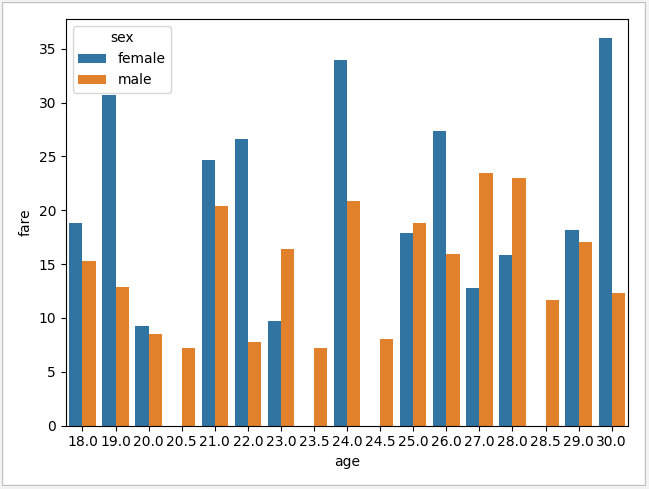
\includegraphics[width=0.7\textwidth]{appendix/cp6/titanic-chart.png}
\end{center}


\begin{center}
\rule{10cm}{0.4pt}
\end{center}
  


\textbf{Resources}

\begin{itemize}
    \item \href{https://pandas.pydata.org/docs/getting_started/intro_tutorials/02_read_write.html}{How do I read and write tabular data?}
    \item \href{https://pandas.pydata.org/docs/getting_started/intro_tutorials/03_subset_data.html}{How do I select a subset of a DataFrame?}
    \item \href{https://pandas.pydata.org/docs/reference/index.html}{API reference pandas.core.groupby}
    \item \href{https://seaborn.pydata.org/generated/seaborn.barplot.html}{API reference seaborn.barplot}
    \item \href{https://cmdlinetips.com/2019/07/how-to-select-rows-of-pandas-dataframe-with-query-function/}{Pandas query(): How to Filter Rows of Pandas Dataframe?}
    \item \href{https://seaborn.pydata.org/generated/seaborn.barplot.html}{How to Make a Seaborn Barplot}
    \item \href{https://www.delftstack.com/howto/python-pandas/how-to-filter-dataframe-rows-based-on-column-values-in-pandas/}{Filter Dataframe Rows Based on Column Values in Pandas}
    \item \href{https://stackoverflow.com/questions/32908315/could-not-interpret-input-error-with-seaborn-when-plotting-groupbys}{'Could not interpret input' error with Seaborn when plotting groupbys}
    \item \href{https://stackoverflow.com/questions/51866908/difference-between-as-index-false-and-reset-index-in-pandas-groupby}{Difference between "as\_index = False", and "reset\_index()" in pandas groupby}
    \item \href{https://stackoverflow.com/questions/32400867/pandas-read-csv-from-url}{Pandas read\_csv from url}
\end{itemize}

\end{scriptsize}
\end{mdframed}
\caption{Description for the Titanic task}
\end{figure}

    